\section{Rehmann theorem for Laurent polynomials}
Let $A$ be arbitrary commutative unital ring and $\mathfrak{m}$ be its ideal.
Denote by $B$ the subring $\mathfrak{m}[t^{-1}] + A[t]$ of the Laurent polynomial ring $A[t, t^{-1}]$ with the $\mathbb{Z}$-grading induced by the grading on $A[t, t^{-1}]$.
As an additive group $B$ decomposes into a direct sum of its homogeneous components $\oplus_{k\in\mathbb{Z}} B_k$,
 where each $B_k \subseteq B$ is equal either to $A\cdot t^k$ for $k \geq 0$ or to $\mathfrak{m} \cdot t^k$ for $k<0$.
  
For $m \geq 1$ consider the following set of Steinberg generators:
\[\XX{m} = \{ x_{\alpha}(\xi) \mid \xi \in B_d,\text{ for } d\leq m,\ \alpha\in\Phi\}. \]
Clearly, $\XX{m} \subseteq \XX{m+1}$, denote by $\XX{\infty}$ the union of all $\XX{n}$'s.

Let $\Phi$ be a reduced irreducible root system of rank $\geq 3$.
The main result of this section is~\cref{prop:tul3.3} which gives a presentation of Steinberg group $\St(\Phi, B)$ in terms of generating set $\mathcal{X}_1$.
In the sequel we will need this presentation only in the special case $\Phi=\rA_3$. However, we preferred to prove a more general statement since the proof in the special case $\Phi=\rA_3$ would have almost the same length.

This presentation given by~\cref{prop:tul3.3} can be thought of as an analogue of~\cite[Lemma~3.3]{Tu83} in the case $n=4$ (with variables $t$ and $t^{-1}$ swapped).
Notice that Tulenbaev's short proof of \cite[Lemma~3.3]{Tu83} in the case $\Phi=\rA_\ell$, $\ell\geq 4$ does not work in the case $\Phi=\rA_3$, which forces us to recourse to a much longer argument inspired by the proof of Rehmann--Soul{\'e} theorem on finite presentation of Steinberg groups over polynomial rings (cf.~\cite{Re75, RS76}).
 
\begin{rem}
There are several reasons why we can not simply refer to~\cite{Re75} or~\cite{RS76} and instead need to reprove everything by hand.
\begin{itemize}
 \item Rehmann and Soul{\'e} deal with usual polynomial rings rather than $\mathbb{Z}$-graded rings
  (i.\,e. their results correspond to the special case $\mathfrak{m}=0$ of our result);
 \item Presentations from~\cite{Re75,RS76} are given in terms of generating set $\XX{2}$ rather than $\mathcal{X}_1$ which is not precise enough for our purposes;
 \item It is assumed that $A=k$ is a field in~\cite{Re75} and that $A=\mathbb{Z}$ in~\cite{RS76}, while our theorem should work with a general coefficient ring $A$.
\end{itemize} 
\end{rem}

We need one additional technical definition. We call an ordered triple of roots $(\alpha, \beta, \gamma) \in \Phi^3$ an {\it $\rA_3$-triple}
 if these vectors form a basis of a root subsystem $\Psi \subseteq \Phi$ of type $\rA_3$, and moreover if the Dynkin diagram of $\Psi$ with respect to this basis has the form
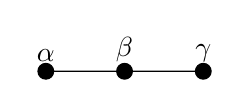
\begin{tikzpicture}
\draw[fill=black] 
(0,0) circle [radius=.1] node [above] {$\alpha$} --
(1,0) circle [radius=.1] node [above] {$\beta$} --
(2,0) circle [radius=.1] node [above] {$\gamma$};
\end{tikzpicture}.
  
For $m\geq 2$ define $G_m$ as the group presented by generators $\mathcal{X}_m$ and the following three families of relations:
\begin{align}
 \label{eq:am} \tag{$a_m$} x_{\alpha}(\xi) x_{\alpha}(\eta) & = x_{\alpha}(\xi+\eta),&  \xi,\eta\in B_d,\ d\leq m;&\\
 \label{eq:bm} \tag{$b_m$} [x_\alpha(\xi), x_{\alpha'}(\eta))] &  = 1, & \text{in the case $\alpha+\alpha'\not\in\Phi\cup\{0\}$,}\\
 \nonumber                                                     &       & \xi \in B_d,\ \eta \in B_e,\ d,e\leq m;\\
 \label{eq:cm} \tag{$c_m$} [x_\alpha(\xi), x_{\alpha'}(\eta)] & = x_{\alpha+\alpha'}(N_{\alpha,\alpha'}\xi\eta), & \text{in the case $\alpha+\alpha'\in \Phi$,}\\
 \nonumber                                                    &  & \xi \in B_d,\ \eta \in B_e,\ d, e, d+e \leq m.
 \end{align}
For $m=1$ define $G_1$ as the group presented by generators $\mathcal{X}_1$, 
three above families of relations $(a_1), (b_1), (c_1)$ and the following additional family:
\begin{align}  \label{eq:d1} \tag{$d_1$} [[x_{\alpha+\beta+\gamma}(\xi), x_{-\gamma}(\eta)], x_{\beta+\gamma}(\zeta) ] & = 1, 
 & \xi,\eta,\zeta\in B_1,\ \text{ $(\alpha, \beta, \gamma)$ is an $\rA_3$-triple. }
\end{align}

The obvious embedding of generators $\mathcal{X}_m \subseteq \mathcal{X}_{m+1}$ induces a map $f_m\colon G_m \to G_{m+1}$.
Our goal is to show the following result.
\begin{prop}\label{prop:tul3.3}
 For $m\geq 1$ the map $f_m$ is an isomorphism. Consequently, $\St(\Phi, B)$ can be presented by generators $\mathcal{X}_1$ and relations $(a_1)$, $(b_1)$, $(c_1)$, $(d_1)$.
\end{prop}
\begin{rem}
   Notice that for $\Phi=\rA_\ell$, $\ell\geq 4$ the group $\St(\Phi, B)$ admits a shorter presentation with family~ $(d_1)$ omitted (see~\cite[Lemma~3.3]{Tu83}).
   This is also true for $\Phi=\rE_\ell$ since $\St(\rE_\ell, R)$ can be presented as an amalgamated product of several copies of $\St(\rA_4, R)$, (cf. e.\,g.~\cite[Lemmas~3,7)]{S15}).   
  On the other hand, we believe that the above presentation is the shortest possible in the cases $\Phi=\rA_3, \rD_\ell$. \end{rem}

We will use the following commutator identities (cf.~\cite[H1]{Re75}):
\begin{align}
 \label{eq:H1ii}  [ab, c] = {}^a[b, c] \cdot [a,c];&\\ %= [a,[b,c]]\cdot [b,c] \cdot [a,c];&\\
 \label{eq:H1iii} [a,c]   = 1    \text{ implies } [a, [b,c]] = [[a,b],{}^bc].&
\end{align}

\begin{lemma}
 Suppose $m \geq 1$.
 Let $\alpha, \beta, \alpha', \beta' \in \Phi$ be such that $\alpha + \beta = \alpha' + \beta'$.
 Assume, moreover, that $\xi \in B_d$, $\xi' \in B_{d'}$, $\eta \in B_e$, $\eta' \in B_{e'}$ are such that 
  $N_{\alpha, \beta} \xi \eta = N_{\alpha', \beta'}\xi' \eta'$ for some $d,d',e,e'\leq m$ satisfying $d+e=d'+e' = m+1$.
 Then the following relations holds in $G_m$:
 \begin{equation}
  \label{eq:S-correctness} [x_\alpha(\xi), x_\beta(\eta)] = [x_{\alpha'}(\xi'), x_{\beta'}(\eta')].
 \end{equation}
 Moreover for every $\zeta \in B_{k''}$, $k''\leq m$ and $\gamma\in\{\alpha, \beta, \alpha + \beta\}$
  the following relation holds in $G_m$:
 \begin{equation}
 \label{eq:S-commutes} [[x_\gamma(\zeta), [x_\alpha(\xi), x_\beta(\eta)]] = 1.
 \end{equation}
\end{lemma}
\begin{proof}
 Notice that $k+l = m+1$, $k, l\leq m$ imply $k,l>0$, hence $B_i= A \cdot t^i$ for $i=k,k',l,'l'$.
 This means that without loss of generality we may assume that $\mathfrak{m}=0$ and $B = A[t]$.
 But now our statement is not different from~\cite[Proposition 1.1]{Re75} (or~\cite[Proposition~3.2.2]{RS76} in the case $g=1$)
  and can be proved by the same argument which remains valid for a general coeffient ring $A$.
\end{proof}

For every $\xi \in B_{m+1}$ and $\alpha\in \Phi$ there exist $\xi' \in B_m$ and $\alpha'\in \Phi$ such that $\xi = t\xi'$ and $\alpha-\alpha'\in\Phi$,
so we can define the following element of $G_m$:
\begin{equation} \label{eq:S-definition} S_\alpha(\xi) := [x_{\alpha-\alpha'}(N_{\alpha-\alpha',\alpha'} \xi'), x_{\alpha'}(t)].\end{equation} 
From~\eqref{eq:S-correctness} it follows that $S_\alpha(\xi)$ does not depend of the choice of $\alpha'$.

Let us show that elements $S_\alpha(\xi)$ satisfy the relations $(a_{m+1})$, $(b_{m+1})$ and $(c_{m+1})$.
From \eqref{eq:H1ii} and~\eqref{eq:S-commutes} it follows that $S_\alpha(\xi)$ satisfy $(a_{m+1})$ and hence $(b_{m+1})$ in the special case $\alpha=\alpha'$.
\begin{lemma} \label{lem:cm-plus1} Suppose that $m\geq 1$. For every $\alpha, \alpha' \in \Phi$ such that $\alpha+\alpha' \in \Phi$ and
 $a\in A$, $\xi \in B_d$, $d \leq 0$ the following relation holds in $G_m$: 
\begin{equation} \nonumber
[x_\alpha(\xi), S_{\alpha'}(at^{m+1})] = [x_\alpha(t\xi), x_{\alpha'}(at^m)] = S_{\alpha+\alpha'}(N_{\alpha,\alpha'}a\xi t^{m+1}).
\end{equation}
\end{lemma}
\begin{proof}
By \cite[Lemma~3.1.2]{RS76} we may assume without loss of generality that $\alpha'=\beta$ for some $\rA_3$-triple $(\alpha, \beta, \gamma)$.
\begin{align*}
   [x_\alpha(\xi), S_\beta(at^{m+1})] = [x_\alpha(\xi), [x_{\beta + \gamma}(t), x_{-\gamma}(a't^m)]]
   &  \text{ by~\eqref{eq:S-correctness},\eqref{eq:S-definition} for $a' = N_{\beta+\gamma, -\gamma} a$} \\ 
 = [x_{\alpha+\beta+\gamma}(\epsilon t\xi), {}^{x_{\beta+\gamma}(t)}x_{-\gamma}(a't^m)]             
 &  \text{ by~\eqref{eq:H1iii}, for $\epsilon=N_{\alpha, \beta+\gamma}$} \\
 = {}^{x_{\beta+\gamma}(t)}[x_{\alpha+\beta+\gamma}(\epsilon t\xi), x_{-\gamma}(a't^m)]             
 &  \text{ by $(b_1)$}
\end{align*} 
Denote by $R$ the expression in the right hand side of the above formula.
\begin{enumerate}
 \item \label{case:cm-1} Case $m=1$, $d = 0$.
 \begin{align*}
   R  = [x_{\alpha +\beta + \gamma}(\epsilon t\xi), x_{-\gamma}(a't)] 
   & \text{ by $(d_1)$}\\
      = {}^{x_{\beta+\gamma}(1)}[x_{\alpha +\beta + \gamma}(\epsilon t\xi), x_{-\gamma}(a't)] 
   & \text{ by~\eqref{eq:H1ii}, $(b_1)$, $(c_1)$} \\
      = [x_\alpha(\xi), [x_{\beta + \gamma}(1), x_{-\gamma}(a't^m)]] 
   & \text{ by $(b_1)$, \eqref{eq:H1iii}}\\
      = [x_\alpha(t\xi), x_\beta(at)]
   & \text{ by~\eqref{eq:S-correctness},\eqref{eq:S-definition}.}
 \end{align*}  
 \item \label{case:cm-2} Case $m\geq 2$ or $m=1$, $d < 0$.
 \begin{align*}
 R = {}^{x_{\beta+\gamma}(t)}[x_{\alpha+\beta+\gamma}(\epsilon t^2\xi), x_{-\gamma}(a't^{m-1})]     
 &  \text{ by~\eqref{eq:S-correctness} if $k=0$ or~\eqref{eq:cm} if $k <0$} \\
 = [[x_\alpha(t\xi), x_{\beta+\gamma}(t)], {}^{x_{\beta+\gamma}(t)} x_{-\gamma}(a't^{m-1})]         
 &  \text{ by~$(b_2)$, $(c_2)$ or by~\eqref{eq:S-commutes},\eqref{eq:S-definition} if $m=1$} \\
 = [x_\alpha(t\xi), x_\beta(at^m)]                                                                  
 &  \text{ by~\eqref{eq:H1iii}. \qedhere}
\end{align*} 

\end{enumerate}
\end{proof}

It will be convenient for us to extend the definition of $S_\alpha(\xi)$ by allowing $\xi$ to take values in $B_d$ for $d\leq m$.
In this case we simply set $S_\alpha(\xi) = x_\alpha(\xi)$.

Now suppose  $0 \leq d \leq m+1$. Clearly \eqref{eq:S-correctness} and \eqref{eq:S-definition} (in the case $1\leq d\leq m$) or~\cref{lem:cm-plus1} (in the case $d=0,m+1$) imply that
\begin{equation} \label{eq:cm-plus1-generalized} 
[S_\alpha(\xi), S_{\alpha'}(\eta)] = S_{\alpha+\alpha'}(N_{\alpha,\alpha'}\xi \eta),\ \xi \in B_d, \eta \in B_{m+1-d}.
\end{equation}

We need to introduce additional notation.
For $a,b\leq m+1$ we denote by $\bot(a, b)$ (resp. $\angle(a,b)$) the family of all relations $[S_\alpha(\xi), S_{\alpha'}(\eta)] = 1$
for which $\xi \in B_a$, $\eta \in B_b$ and $\alpha$ and $\alpha'$ are orthogonal (resp. form a sharp angle). 
We denote by $\bot_0(a, b)$ the subset of $\bot(a, b)$
consisting of those relations for which $\xi = t^{a} \in B_a$.

\begin{lemma} \label{claim1} In $G_m$ relations $\bot_0(1, d)$ and $\angle(d, m)$ imply $\angle(d, m+1)$ for $d\leq m+1$ \end{lemma}
\begin{proof}
Without loss of generality we may assume that $\alpha' = \alpha + \beta$
  for some $\rA_3$-triple $(\alpha, \beta, \gamma)$.
Write $\eta = bt^{m+1}$ for some $b\in A$.
\begin{align*} 
[S_\alpha(\xi), S_{\alpha+\beta}(bt^{m+1})] = [S_\alpha(\xi), [x_{\alpha+\beta+\gamma}(b't^m), x_{-\gamma}(t)]] & \text{ by~\eqref{eq:S-correctness} and~\eqref{eq:S-definition}}\\
= [[S_\alpha(\xi), x_{\alpha+\beta+\gamma}(b't^m)], {}^{x_{\alpha+\beta+\gamma}(b't^m)}\!x_{-\gamma}(t)] & \text{ by~$\bot_0(1, d)$}\\
= 1
 & \text{ by~$\angle(d, m)$. \qedhere} \end{align*} 
\end{proof}

\begin{lemma} \label{claim2} In $G_m$ relations $\angle(d, m+1)$ imply $\bot_0(d, m+1)$ for  $1\leq d\leq m+1$. \end{lemma}
\begin{proof}
As before, without loss of generality we may assume $\alpha' = \gamma$ for some $\mathsf{A}_3$-triple $(\alpha, \beta, \gamma)$.
 \begin{align*}
 {}^{S_\gamma(t^d)}S_\alpha(bt^{m+1}) = {}^{S_\gamma(t^d)}[S_{-\beta}(b't^{m+1}), x_{\alpha+\beta}(1)] & \text{ by~\cref{lem:cm-plus1}}\\
 = [S_{-\beta}(b't^{m+1}), {}^{S_\gamma(t^d)}x_{\alpha+\beta}(1)]                                     
 & \text{ by $\angle(d, m+1)$}\\
 = [[x_{-\beta-\gamma}(b''t^{m+1-d}), S_\gamma(t^d)], {}^{S_\gamma(t^d)}x_{\alpha+\beta}(1)]          
 & \text{ by~\eqref{eq:cm-plus1-generalized}}\\
 = [x_{-\beta-\gamma}(b''t^{m+1-d)}), [S_\gamma(t^d), x_{\alpha+\beta}(1)]]                           
 & \text{ by~\eqref{eq:H1iii} and $(b_{m+1-d})$}\\
 = S_{\alpha}(b'''t^{m+1})                                                                            
 & \text{ by~\eqref{eq:cm-plus1-generalized}.} \end{align*}
Usual identities for structure constants imply (cf.~\cite[p.~12]{Re75}):
 $b'''=N_{-\beta-\gamma, \alpha+\beta+\gamma} \cdot N_{\gamma, \alpha+\beta} \cdot N_{-\beta-\gamma, \gamma} \cdot N_{-\beta, \alpha+\beta} \cdot b = b,$ from which the claim follows.
\end{proof}

\begin{lemma} \label{claim3}
 In $G_m$ relations $\bot_0(d, m+1)$, $\angle(d, d)$ and $\angle(m+1, m+1)$ imply $\bot(d, m+1)$ for $d\leq m+1$.
\end{lemma}
\begin{proof}
 \begin{align*} 
 S_{\alpha+\beta+\gamma}(abt^{m+1}) = {}^{S_{-\beta}(t^d)}\!S_{\alpha+\beta+\gamma}(abt^{m+1}) 
 & \text{ by $\bot_0(d, m+1)$}\\
 = {}^{S_{-\beta}(t^d)}\![x_{\alpha+\beta}(b't^{m+1-d}), S_\gamma(at^d)] 
 & \text{ by~\eqref{eq:cm-plus1-generalized}} \\
 = [S_{\alpha}(b't^{m+1}) x_{\alpha+\beta}(b't^{m+1-d}), S_\gamma(at^d)] 
 & \text{ by~\eqref{eq:cm-plus1-generalized} and $\angle(d, d)$ }\\
 = {}^{S_{\alpha}(b't^{m+1})}\!S_{\alpha+\beta+\gamma}(abt^{m+1}) [S_{\alpha}(b't^{m+1}), S_\gamma(at^d)] 
 & \text{ by~\eqref{eq:H1ii} and~\eqref{eq:cm-plus1-generalized}} \\
 = S_{\alpha+\beta+\gamma}(abt^{m+1}) [S_{\alpha}(b't^{m+1}), S_\gamma(at^d)] 
 & \text{ by $\angle(m+1, m+1)$. \qedhere}
\end{align*}
\end{proof}

\begin{lemma} \label{lem:bm-plus1}
Elements $S_\alpha(\xi)$ satisfy relations $(b_{m+1})$.
 \end{lemma}
\begin{proof}
We must show that $S_\alpha(\xi)$ satisfy $\angle(d, m+1)$ and $\bot(d, m+1)$ for $d\leq m+1$.
\begin{enumerate}
 \item Relations $\angle(d, m+1)$, $d\leq m$ follow from~\cref{claim1}. 
 \item Relations $\bot(d, m+1)$ with $d\leq 0$ can verified by direct computation:
 \begin{align*} 
 [x_\alpha(\xi), S_{\gamma}(bt^{m+1})] = [x_\alpha(\xi), [x_{\beta+\gamma}(b't^m), x_{-\beta}(t)]] & \text{ by~\eqref{eq:S-correctness},\eqref{eq:S-definition}} \\
 = [[x_\alpha(\xi), x_{\beta+\gamma}(b't^m)], {}^{x_{\beta+\gamma}(b't^m)}\!x_{-\beta}(t)] &
 \text{ by \eqref{eq:H1iii} and $(b_1)$} \\
 = {}^{x_{\beta+\gamma}(b't^m)}\![x_{\alpha+\beta+\gamma}(b't^m\xi), x_{-\beta}(t)] &
 \text{ by $(b_m)$ and $(c_m)$} \\
 = 1 & \text{ by $(b_m)$.}
\end{align*}
 \item Relations $\bot_0(d, m+1)$ with $1\leq d\leq m$ follow from~\cref{claim2}.
 \item Relations $\angle(m+1, m+1)$ follow from~\cref{claim1}, consequently relations $\bot_0(m+1, m+1)$ follow from~\cref{claim2}.
 \item Relations $\bot(d, m+1)$, $0\leq d\leq m+1$ follow from~\cref{claim3} and the previous two assertions.
\end{enumerate}
\end{proof}

\begin{proof}[Proof of~\cref{prop:tul3.3}]
Define the map $g_m\colon G_{m+1} \to G_m$ by $g_m(x_\alpha(\xi)) = S_\alpha(\xi)$.
In view of the above lemmata this map is well-defined. It is clear that $g_m$ is inverse to $f_m$, which proves the first claim.

Denote by $G_\infty$ the group presented by generators $\mathcal{X}_\infty$ and relations $(a_\infty)$, $(b_\infty)$, $(c_\infty)$.
By the above argument there is an isomorphism between $G_1$ and $\colim\limits_{n\to\infty} G_n \cong G_\infty$.

Denote by $i\colon G_\infty \to \St(\Phi, B)$ the map induced by the obvious embedding of $\mathcal{X}_\infty$ into the set of 
 Steinberg generators of $\St(\Phi, B)$.  
Using~\eqref{eq:H1ii} multiple times it is not hard to show that the map $j\colon \St(\Phi, B) \to G_\infty$ given by
 $j(x_\alpha(b)) = \prod x_\alpha(b_i)$, where $b = \sum b_k$ is the decomposition of $b$ into a finite sum of its homogeneous components $b_k\in B_k$, is a well-defined map.
It is clear that $i$ and $j$ are mutually inverse. 
\end{proof}
